\hyphenation{
Bonfatti
}


\documentclass[a4paper, 12pt]{article}
\usepackage{fancyhdr}
\pagestyle{fancy}
% i comandi seguenti impediscono la scrittura in maiuscolo
% dei nomi dei capitoli e dei paragrafi nelle intestazioni
%\renewcommand{\chaptermark}[1]{\markboth{#1}{}}
%\renewcommand{\sectionmark}[1]{\markright{\thesection\ #1}}
%\fancyhf{} % rimuove l’attuale contenuto dell’intestazione
%% e del pi\‘e di pagina
%\fancyhead[LE,RO]{\bfseries\thepage}
%\fancyhead[LO]{\bfseries\rightmark}
%\fancyhead[RE]{\bfseries\leftmark}
%\renewcommand{\headrulewidth}{0.5pt}
%\renewcommand{\footrulewidth}{0pt}
%\addtolength{\headheight}{0.5pt} % riserva spazio per la linea
%\fancypagestyle{plain}{%
%\fancyhead{} % ignora, nello stile plain, le intestazioni
%\renewcommand{\headrulewidth}{0pt} % e la linea
%}
\usepackage[italian]{babel}
\usepackage[utf8]{inputenc}
\usepackage{graphicx}
\usepackage{amsthm}
\usepackage{vhistory}
\usepackage{hyperref}

\title{Differenze tra primo e secondo schiacciatore}
\author{
Mattia Natale\footnote{
http://www.andrea-asta.com/volleyworld/2007/10/27/differenze-tra-primo-e-secondo-schiacciatore/}
}
\date {}

\frenchspacing


\theoremstyle{remark}
\newtheorem*{nota}{Nota}

\theoremstyle{definition}
\newtheorem{defi}{Definizione}

\begin{document}
\maketitle

Molti si chiedono quale sia la differenza fra prima e seconda banda, primo o secondo centro. Pochi lo sanno o ci hanno perso dieci minuti per capirlo. Oggi mi occuperò delle differenze che si rilevano fra le due bande in campo.

\section{Analisi delle rotazioni}

Analizziamo giro per giro i compiti di entrambe le bande.

\[
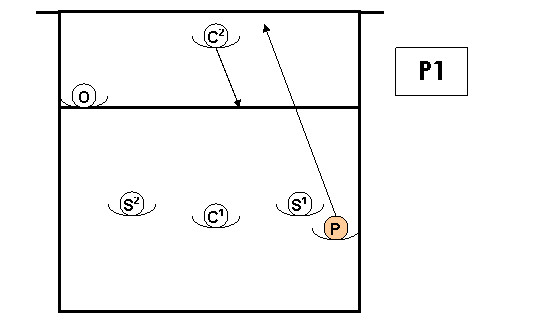
\includegraphics[scale=.65]{img/image01.jpg}
\]

Partiamo dalla P1. Il primo schiacciatore (che d’ora in poi chiamerò S1) si trova in zona 2. Di conseguenza il secondo schiacciatore (che chiamerò S2) si trova in zona 5. Partiamo dalla fase CP (Cambio palla, cioè siamo in ricezione): S1 scenderà in zona 1 per fare penetrare il palleggiatore, S2 riceverà in zona 5.
In fase di attacco il primo schiacciatore attaccherà in rotazione in cui avremo tre attaccanti in prima linea (da ora in avanti, per comodità, ci riferiremo a questa situazione con l’espressione “in attacco a 3“) ed il secondo centrale in prima linea.
Con palla nel campo avversario S1 murerà la banda dell’altra squadra e S2 coprirà l’entrata del palleggiatore.

\[
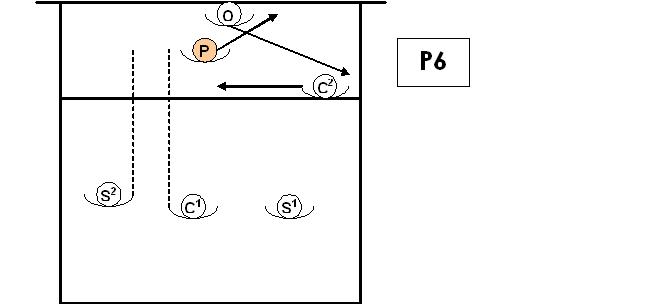
\includegraphics[scale=.85]{img/image02.jpg}
\]

P6: S1 riceverà ancora in zona 1 e S2 scenderà in zona 5. Uguale a prima. In fase di attacco avremo attacco a tre con il secondo centrale davanti. S1 dovrà coprire l’entrata del palleggiatore.

\[
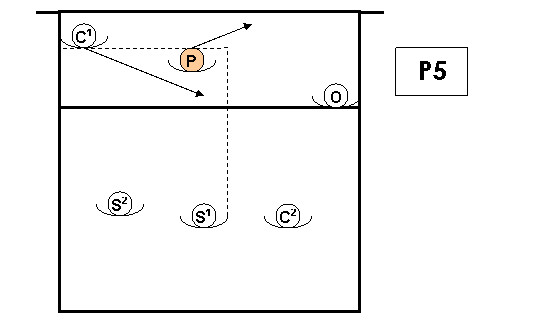
\includegraphics[scale=.65]{img/image03.jpg}
\]

P5: S2 scenderà ancora una volta in zona 5, mentre S1 riceverà in zona 6. S2 schiaccerà in attacco a 3 con il primo centrale davanti. S1 dovrà ancora una volta coprire l’entrata del palleggiatore.

\[
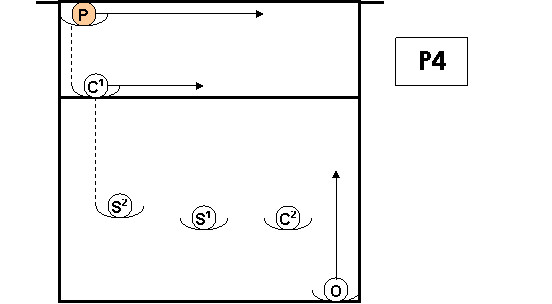
\includegraphics[scale=.65]{img/image04.jpg}
\]

P4: S2 riceverà sempre in zona 5 e S1 in zona 6, come nel giro precedente. Questa volta avremo un attacco a 2, quindi S2 si troverà ad attaccare insieme al primo centrale. Il palleggiatore è in prima linea quindi S1 non dovrà coprirne l’entrata.

\[
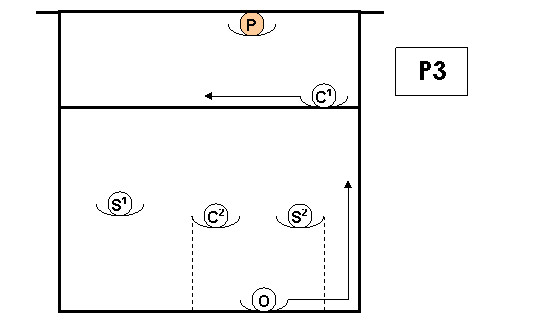
\includegraphics[scale=.65]{img/image05.jpg}
\]

P3: S1 si trova in prima linea quindi in questo giro dovrà ricevere in zona 5, mentre S2 che ha terminato i suoi tre giri in prima linea riceverà in zona 1. S1 schiaccerà con attacco a 2 e il primo centrale davanti.

\[
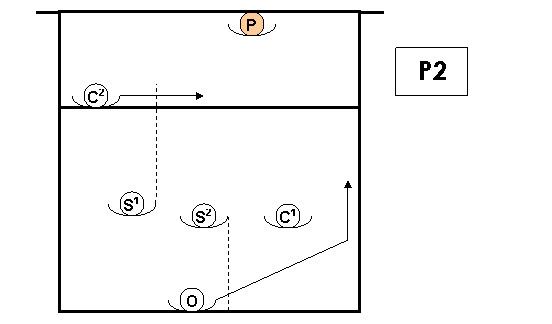
\includegraphics[scale=.65]{img/image06.jpg}
\]

P2: Ultimo giro da descrivere. S1 è ancora in prima linea e scenderà a ricevere in zona 5, mentre S2 che si trova in zona 6 dovrà rimanere in tale zona a ricevere. Avremo attacco a 2 per S1 affiancato dal secondo centrale.

\section{Qualche conslusione}

Ora che abbiamo esaminato tutti i giri possiamo iniziare a trarre qualche conclusione.

    S1 riceve, in ordine di enunciazione in zone: 1,1,6,6,5,5. Quindi riceverà due volte in ogni zona;
    S2 riceve, sempre in ordine di enunciazione in zone: 5,5,5,5,1,6. Ovvero riceverà la maggior parte delle volte in zona 5;
    S1 dovrà coprire due volte l’entrata del palleggiatore, mentre toccherà solo una volta al S2 svolgere questo compito;
    S1 schiaccerà due volte con attacco a 2, mentre S2 una volta sola;
    S1 dovrà attaccare due volte affiancato dal secondo centrale e una volta dal primo, mentre si inverte la situazione per S2.

Questo è in linea generale, ma andiamo a vedere effettivamente cosa cambia.

Ritengo che la ricezione da zona 6 sia la più semplice in quanto la palla arriva quasi sempre frontale. L’ unico handicap è che abbiamo due zone di conflitto, sia a sinistra che a destra. La ricezione da zona 1 è forse la più problematica, soprattutto per chi usa il “metodo della priorità a sinistra”, cioè su una palla che arriva in mezzo a due ricevitori, dovrebbe riceverla il giocatore a destra. Facendo questo il giocatore di zona 1 si trova a coprire più campo (sia un po’ di campo a destra che a sinistra). Anche se, solitamente, la battuta arriva dalla zona 1 opposta e quindi ha anche più tempo per spostarsi. Inoltre aggiungiamo che la ricezione da zona 1 arriva da dietro al palleggiatore. Anche qui la ricezione risulta quasi frontale.

Chi riceve da zona 5 deve anche attaccare. Di norma la battuta gli arriva da zona 1, quindi frontalmente e la ricezione non dovrebbe essere problematica. A parte il fatto che se non si riceve abbastanza alto non si ha il tempo per aprirsi.

Detto questo, credo che i vari pro e contro in ricezione si compensino e che quindi la differenza fra primo e secondo schiacciatore sia minima.

Per la copertura del palleggiatore c’è poco da dire: il primo schiacciatore deve coprire per due giri l’entrata del palleggiatore, mentre il secondo per uno solo. Quindi, in linea teorica, S1 dovrebbe sapere coprire meglio la zona d’entrata, quindi essere più reattivo e forte in difesa/rullata (ricordo che i palloni lunghi in zona 1 da prendere quando il palleggiatore è entrato spesso si possono prendere solo in rullata). Però ricordo anche che, comunque, non avremo decine di questi palloni a partita, quindi anche qui la differenza è irrilevante.

Ora veniamo all’attacco, rivedendo brevemente cosa accade:

    Prima banda
        In P1 schiaccia con attacco a 3 affiancato dal secondo centrale;
        In P3 schiaccia con attacco a 2 affiancato dal primo centrale;
        In P2 schiaccia con attacco a 2 affiancato dal secondo centrale.
    Seconda banda
        In P6 schiaccia con attacco a 3 affiancato dal secondo centrale;
        In P5 schiaccia con attacco a 3 affiancato dal primo centrale;
        In P4 schiaccia con attacco a 2 affiancato dal primo centrale.

Guardando lo schema possiamo dedurre che S1 schiaccia più spesso con attacco a 2 e con il secondo centrale. Approssimando che il primo centrale dovrebbe essere più incisivo in attacco possiamo dedurre che anche il primo schiacciatore dovrebbe esserlo poiché attacca più spesso con attacco a due e con il centrale meno incisivo in attacco. Questa differenza può essere rilevante in squadre di livello medio-basso, poiché ritengo che in squadre a un livello maggiore l’opposto non abbia difficoltà ad attaccare dalla seconda linea (ammesso che per il palleggiatore non sia problematico alzare in seconda linea) e quindi la rilevanza di avere un attacco a due o a tre sia insignificante. Certo, c’è tutto il discorso sul muro da fare, ma ritengo che ad un livello provinciale-regionale non sia così incisivo.

Quindi, teoricamente, il primo schiacciatore dovrebbe essere maggiormente incisivo in attacco, a meno di non avere un buon opposto affiancato da un ottimo palleggiatore, e a questo punto le differenze fra primo e secondo schiacciatore si minimizzerebbero.
\end{document}